% Options for packages loaded elsewhere
\PassOptionsToPackage{unicode}{hyperref}
\PassOptionsToPackage{hyphens}{url}
%
\documentclass[
]{article}
\usepackage{amsmath,amssymb}
\usepackage{lmodern}
\usepackage{ifxetex,ifluatex}
\ifnum 0\ifxetex 1\fi\ifluatex 1\fi=0 % if pdftex
  \usepackage[T1]{fontenc}
  \usepackage[utf8]{inputenc}
  \usepackage{textcomp} % provide euro and other symbols
\else % if luatex or xetex
  \usepackage{unicode-math}
  \defaultfontfeatures{Scale=MatchLowercase}
  \defaultfontfeatures[\rmfamily]{Ligatures=TeX,Scale=1}
\fi
% Use upquote if available, for straight quotes in verbatim environments
\IfFileExists{upquote.sty}{\usepackage{upquote}}{}
\IfFileExists{microtype.sty}{% use microtype if available
  \usepackage[]{microtype}
  \UseMicrotypeSet[protrusion]{basicmath} % disable protrusion for tt fonts
}{}
\makeatletter
\@ifundefined{KOMAClassName}{% if non-KOMA class
  \IfFileExists{parskip.sty}{%
    \usepackage{parskip}
  }{% else
    \setlength{\parindent}{0pt}
    \setlength{\parskip}{6pt plus 2pt minus 1pt}}
}{% if KOMA class
  \KOMAoptions{parskip=half}}
\makeatother
\usepackage{xcolor}
\IfFileExists{xurl.sty}{\usepackage{xurl}}{} % add URL line breaks if available
\IfFileExists{bookmark.sty}{\usepackage{bookmark}}{\usepackage{hyperref}}
\hypersetup{
  pdftitle={World Development Indicators},
  hidelinks,
  pdfcreator={LaTeX via pandoc}}
\urlstyle{same} % disable monospaced font for URLs
\usepackage[margin=1in]{geometry}
\usepackage{graphicx}
\makeatletter
\def\maxwidth{\ifdim\Gin@nat@width>\linewidth\linewidth\else\Gin@nat@width\fi}
\def\maxheight{\ifdim\Gin@nat@height>\textheight\textheight\else\Gin@nat@height\fi}
\makeatother
% Scale images if necessary, so that they will not overflow the page
% margins by default, and it is still possible to overwrite the defaults
% using explicit options in \includegraphics[width, height, ...]{}
\setkeys{Gin}{width=\maxwidth,height=\maxheight,keepaspectratio}
% Set default figure placement to htbp
\makeatletter
\def\fps@figure{htbp}
\makeatother
\setlength{\emergencystretch}{3em} % prevent overfull lines
\providecommand{\tightlist}{%
  \setlength{\itemsep}{0pt}\setlength{\parskip}{0pt}}
\setcounter{secnumdepth}{-\maxdimen} % remove section numbering
\ifluatex
  \usepackage{selnolig}  % disable illegal ligatures
\fi

\title{World Development Indicators}
\author{true}
\date{2022-02-07}

\begin{document}
\maketitle

\hypertarget{background}{%
\section{Background}\label{background}}

The \href{http://www.worldbank.org/}{World Bank} collects statistical
information from countries around the world. A particularly useful data
set is the \textbf{W}orld \textbf{D}evelopment \textbf{I}ndicators
\href{http://data.worldbank.org/data-catalog/world-development-indicators}{(WDI)}
which are country level statistical information from around the world.

Using \texttt{library(WDI)} you can download indicator data directly
from the World Bank, read it into a data set, and put it to use.

\hypertarget{call-libraries}{%
\section{Call Libraries}\label{call-libraries}}

\begin{verbatim}
## Warning: package 'WDI' was built under R version 4.1.2
\end{verbatim}

\begin{verbatim}
## Warning: package 'DT' was built under R version 4.1.2
\end{verbatim}

\begin{verbatim}
## Warning: package 'foreign' was built under R version 4.1.1
\end{verbatim}

\begin{verbatim}
## Warning: package 'haven' was built under R version 4.1.2
\end{verbatim}

\begin{verbatim}
## Warning: package 'dplyr' was built under R version 4.1.2
\end{verbatim}

\begin{verbatim}
## 
## Attaching package: 'dplyr'
\end{verbatim}

\begin{verbatim}
## The following objects are masked from 'package:stats':
## 
##     filter, lag
\end{verbatim}

\begin{verbatim}
## The following objects are masked from 'package:base':
## 
##     intersect, setdiff, setequal, union
\end{verbatim}

\hypertarget{search-for-indicators}{%
\section{Search For Indicators}\label{search-for-indicators}}

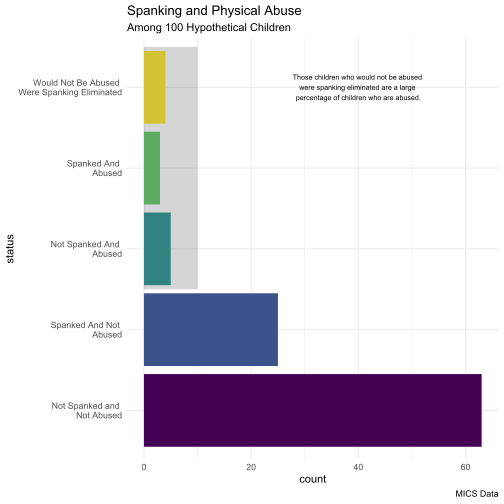
\includegraphics{index_files/figure-latex/unnamed-chunk-3-1.pdf}

\hypertarget{download-data}{%
\section{Download Data}\label{download-data}}

I am guessing that we are most interested in the indicator
\texttt{SP.POP.0305.TO.UN:\ \ Population,\ ages\ 3-5\ total}, but we
could modify this script to get another indicator, or multiple
indicators.

A sample of the data is below, and the full data in various formats can
be found \href{./}{here}.

\begin{verbatim}
##   iso2c                          country SP.POP.0305.TO.UN year status iso3c
## 1       Global Partnership for Education                NA 2025         <NA>
## 2       Global Partnership for Education                NA 2020         <NA>
## 3       Global Partnership for Education                NA 2019         <NA>
## 4       Global Partnership for Education                NA 2018         <NA>
## 5       Global Partnership for Education                NA 2017         <NA>
## 6       Global Partnership for Education                NA 2016         <NA>
##   region capital longitude latitude income lending
## 1   <NA>    <NA>      <NA>     <NA>   <NA>    <NA>
## 2   <NA>    <NA>      <NA>     <NA>   <NA>    <NA>
## 3   <NA>    <NA>      <NA>     <NA>   <NA>    <NA>
## 4   <NA>    <NA>      <NA>     <NA>   <NA>    <NA>
## 5   <NA>    <NA>      <NA>     <NA>   <NA>    <NA>
## 6   <NA>    <NA>      <NA>     <NA>   <NA>    <NA>
\end{verbatim}

\end{document}
